% !TEX root = task-1-13-5.tex
% Editable task bank. Append new BankTask blocks at the end of the document.
\documentclass[12pt,a4paper]{article}
\usepackage{physics-textbook}
\usepackage{graphicx,needspace}
\usetikzlibrary{decorations.pathmorphing}
\newif\ifShowSolutions
\ifdefined\TutorEdition
  \ShowSolutionstrue
\else
  \ShowSolutionsfalse % Change to \ShowSolutionstrue to display solutions.
\fi
\newcounter{banktask}
\newsavebox{\BankTaskBox}
\newcommand{\BankTaskContent}[3]{%
  \noindent\textbf{\thebanktask.}\quad #2\par
  \ifShowSolutions
    \Needspace{50mm}% Keep the solution heading with its opening text or diagram.
    #3\par
    \ifdefined\TutorEdition
      \ifcsname TutorSource#1\endcsname
        \nopagebreak\smallskip{\small\csname TutorSource#1\endcsname\par}%
      \fi
    \fi
  \fi
}
\newcommand{\BankTask}[3]{%
  \refstepcounter{banktask}\par\medskip
  \sbox{\BankTaskBox}{\begin{minipage}{\linewidth}%
    \BankTaskContent{#1}{#2}{#3}\end{minipage}}%
  \ifdim\dimexpr\ht\BankTaskBox+\dp\BankTaskBox\relax>\dimexpr\textheight-20mm\relax
    \Needspace{35mm}\BankTaskContent{#1}{#2}{#3}%
  \else
    \Needspace{\dimexpr\ht\BankTaskBox+\dp\BankTaskBox\relax}%
    \noindent\usebox{\BankTaskBox}\par
  \fi
  \medskip
}
\begin{document}
\BookSubsection{1.13.5}{Плавание тел}


% Source sdamgia-3470: https://phys-ege.sdamgia.ru/problem?id=3470
\BankTask{sdamgia-3470}{
На поверхности воды плавает брусок массой $50\,\text{г}$. Чему равна выталкивающая сила, действующая на брусок, и как она направлена?\begin{enumerate}\item $0{,}5\,\text{Н}$; вниз.\item $0{,}5\,\text{Н}$; вверх.\item $50\,\text{Н}$; вниз.\item $500\,\text{Н}$; вверх.\end{enumerate}
}{
\smallskip\noindent\textbf{Решение}\par
На плавающий брусок действует две силы: сила тяжести и выталкивающая сила Архимеда. Поскольку брусок покоится, согласно второму закону Ньютона, эти силы уравновешены. Следовательно, выталкивающая сила направлена вверх и равна по величине силе тяжести, действующей на брусок $F_{\text{выт}}=mg=0{,}05\,\text{кг}\cdot10\,\text{м/с}^2=0{,}5\,\text{Н}.$
Ответ: $2$.
}

% Source sdamgia-28078: https://phys-ege.sdamgia.ru/problem?id=28078
\BankTask{sdamgia-28078}{
Полый стальной шар массой $8\,\text{кг}$ плавает на поверхности озера. Объем шара равен $16\,\text{дм}^3$. Чему равна сила Архимеда, действующая на шар?
}{
\smallskip\noindent\textbf{Решение}\par
Поскольку по условию задачи шар плавает, то выполняется условие плавания тел: $F_A=mg=8\,\text{кг}\cdot10\,\text{м/с}^2=80\,\text{Н}.$ 
 
Ответ: $80$.
}

% Source sdamgia-41538: https://phys-ege.sdamgia.ru/problem?id=41538
\BankTask{sdamgia-41538}{
Сплошной кубик из железа плавает в ртути. Ребро кубика равно $10\,\text{см}$. Определите силу Архимеда, действующую на кубик.
}{
\smallskip\noindent\textbf{Решение}\par
Так как тело плавает, то $F_A=mg=\rho_{\text{ж}}ga^3=7800\cdot10\cdot0{,}1^3=78\,\text{Н}.$
 
Ответ: $78$.
}

% Source sdamgia-32281: https://phys-ege.sdamgia.ru/problem?id=32281
\BankTask{sdamgia-32281}{
Два одинаковых бруска толщиной $10\,\text{см}$ каждый, связанные друг с другом, плавают в воде так, что уровень воды приходится на границу между ними (см. рис.). На сколько увеличится глубина погружения стопки брусков, если в нее добавить еще один такой же брусок?\par\begin{center}\begin{tikzpicture}[book diagram,scale=.8]
\fill[cyan!25] (0,0) rectangle (3,2);\draw (0,3.1)--(0,0)--(3,0)--(3,3.1);
\draw[cyan!70!black] (0,2)--(3,2);\draw[fill=orange!25] (.4,1.6) rectangle (2.6,2.4);
\end{tikzpicture}\end{center}\par
}{
\smallskip\noindent\textbf{Решение}\par
Если считать два связанных бруска как одно тело, то из условия следует, что это тело при плавании погружено наполовину. При этом глубина погружения равна $10\,\text{см}$. Тогда при добавлении еще одного такого же бруска, новое тело будет погружено наполовину, то есть глубина погружения станет равной $15\,\text{см}$, то есть изменится на $5\,\text{см}$.
 
Ответ: $5$.
}

% Source sdamgia-7345: https://phys-ege.sdamgia.ru/problem?id=7345
\BankTask{sdamgia-7345}{
Кубик из пробки с ребром $10\,\text{см}$ опускают в воду. Каково отношение объема кубика, находящегося над водой, к объему кубика, находящемуся под водой? Плотность пробки $0{,}25\,\text{г/см}^3$.
}{
\smallskip\noindent\textbf{Решение}\par
На кубик в воде действуют две силы: сила Архимеда и сила тяжести. По второму закону Ньютона: $F_A=F_{\text{т}}$

$\rho_{\text{ж}}gV_{\text{п}}=\rho_{\text{к}}g(V_{\text{п}}+V_{\text{н}}),$

где $V_{\text{п}}$ — объем кубика под водой, $V_{\text{н}}$ — объем кубика над водой, $\rho_{\text{к}}$ — плотность пробки.
Поделим выражение на $V_{\text{п}}$ и выразим $\frac{V_{\text{н}}}{V_{\text{п}}}:$

$\frac{V_{\text{н}}}{V_{\text{п}}}=\frac{\rho_{\text{ж}}}{\rho_{\text{к}}}-1=\frac{1000}{250}-1=3.$

Ответ: $3$.
}

% Source sdamgia-10634: https://phys-ege.sdamgia.ru/problem?id=10634
\BankTask{sdamgia-10634}{
На плавающем в воде теле объемом $500\,\text{см}^3$ стоит кубик массой $100\,\text{г}$. При этом тело погружено в воду целиком, а кубик весь находится над водой. Чему станет равным объем погруженной в воду части тела, если снять с него кубик? В обоих случаях плавание тела является установившимся.
}{
\smallskip\noindent\textbf{Решение}\par
По второму закону Ньютона сила тяжести, которая действует на плавающее тело, уравновешивается силой Архимеда:

$F_{\text{т}}=F_A=\rho_{\text{ж}}gV_{\text{т}}.$

Запишем уравнения для двух случаев:

\[\begin{cases}\rho_{\text{ж}}gV_1=(m_1+m_2)g,\\\rho_{\text{ж}}gV_2=m_1g.\end{cases}\]

Вычтем из верхнего уравнения нижнее и найдем объем погруженной части тела во втором случае:

\[\begin{aligned}g\rho_{\text{ж}}V_1-g\rho_{\text{ж}}V_2&=gm_2,\\V_2&=\frac{g\rho_{\text{ж}}V_1-gm_2}{g\rho_{\text{ж}}}=V_1-\frac{m_2}{\rho_{\text{ж}}}\\&=500\,\text{см}^3-\frac{100\,\text{г}}{1\,\text{г/см}^3}=400\,\text{см}^3.\end{aligned}\]

Ответ: $400$.
}

% Source sdamgia-7692: https://phys-ege.sdamgia.ru/problem?id=7692
\BankTask{sdamgia-7692}{
Пустой цилиндрический стеклянный стакан плавает в воде, погрузившись на половину своей высоты. Дно стакана при плавании горизонтально, плотность стекла $2500\,\text{кг/м}^3$. Чему равно отношение внутреннего объема стакана к его наружному объему?
}{
\smallskip\noindent\textbf{Решение}\par
Обозначим за $V_1$ объем стекла стакана, за $V_2$ объем воздуха в стакане.
На стакан действуют сила тяжести $F_{\text{тяж}}=mg=V_1\rho_{\text{ст}}g$ и сила Архимеда $F_{\text{арх}}=\rho_{\text{в}}g\frac{V_1+V_2}{2}.$
Условие плавания тел: $F_{\text{арх}}=F_{\text{тяж}}.$ Получаем:

$2500gV_1=\frac{1000}{2}g(V_1+V_2),$
 
$\frac{V_1}{V_1+V_2}=\frac{500}{2500}=0{,}2.$

Нужно найти отношение внутреннего объема к внешнему, то есть отношение объема воздуха ко всему объему:

$\frac{V_2}{V_1+V_2}=1-\frac{V_1}{V_1+V_2}=1-0{,}2=0{,}8.$

Ответ: $0{,}8$.
}

% Source sdamgia-2919: https://phys-ege.sdamgia.ru/problem?id=2919
\BankTask{sdamgia-2919}{
Деревянный брусок плавает на поверхности воды в миске. Миска покоится на поверхности Земли. Что произойдет с глубиной погружения бруска в воду, если миска будет стоять на полу лифта, который движется с ускорением, направленным вертикально вверх? Ответ поясните, используя физические закономерности.
}{
\smallskip\noindent\textbf{Решение}\par
$1$. Сила Архимеда, которая поддерживает брусок на поверхности воды, равна по модулю весу вытесненной бруском воды.
$2$. Когда брусок, вода и миска покоятся относительно Земли, одна и та же сила Архимеда уравновешивает силу тяжести, как в случае плавающего бруска, так и в случае вытесненной им воды. Поэтому масса бруска и масса вытесненной им воды одинаковы.
$3$. Когда брусок, вода и миска покоятся относительно друг друга, но движутся с ускорением относительно Земли, одна и та же сила Архимеда вместе с силой тяжести сообщает одно и то же ускорение как плавающему бруску, так и воде в объеме, вытесненном бруском, что приводит к соотношению: $\vec F_A=m(\vec a-\vec g)=m_{\text{вытесн. воды}}(\vec a-\vec g),$ откуда следует, что и при движении относительно Земли с ускорением $\vec a\ne\vec g$ масса бруска и масса вытесненной им воды одинаковы. Поскольку масса бруска одна и та же, масса вытесненной им воды в обоих случаях одинакова. Вода практически несжимаема, поэтому плотность воды в обоих случаях одинакова. Значит, объем вытесненной воды не изменяется, глубина погружения бруска в лифте остается прежней.
}

% Source sdamgia-29999: https://phys-ege.sdamgia.ru/problem?id=29999
\BankTask{sdamgia-29999}{
Плоская льдина плавает в воде, выступая над ее поверхностью на $h=0{,}04\,\text{м}$. Определите массу льдины, если площадь ее поверхности $S=2500\,\text{см}^2$. Плотность льда равна $900\,\text{кг/м}^3$.
}{
\smallskip\noindent\textbf{Решение}\par
\par\begin{center}\begin{tikzpicture}[book diagram,scale=.8]
\fill[cyan!20] (-2,-1.1) rectangle (2,.15);\draw (-2,.15)--(2,.15);
\draw[fill=white] (-1.4,-.7) rectangle (1.4,.8);\node at(-.4,.65){$S$};
\draw[<->] (-1.75,.15)--(-1.75,.8) node[midway,left] {$h$};
\fill (0,0) circle(.025);\draw[->,thick] (0,0)--(0,1.35) node[right] {$\vec F_A$};
\fill(.2,-.2) circle(.025);\draw[->,thick] (.2,-.2)--(.2,-1.25) node[right] {$m\vec g$};
\end{tikzpicture}\end{center}\par

На льдину действуют сила тяжести mg и сила Архимеда $F_A=\rho_{\text{в}}gV_{\text{пчт}},$ где масса льдины $m=\rho_{\text{л}}V,$ объем льдины $V=SH,$ объем погруженной части льдины $V_{\text{пчт}}=S(H-h).$
Так как льдина плавает, то выполняется условие равновесия:

$F_A=mg,$ то есть $\rho_{\text{в}}g(H-h)S=\rho_{\text{л}}gHS,$

 где $\rho_{\text{в}}$ — плотность воды, $H$ — толщина льдины, откуда $H=\frac{\rho_{\text{в}}h}{\rho_{\text{в}}-\rho_{\text{л}}}.$ Следовательно, масса льдины равна

\[\begin{aligned}m&=\rho_{\text{л}}SH=\frac{\rho_{\text{л}}\rho_{\text{в}}Sh}{\rho_{\text{в}}-\rho_{\text{л}}}\\&=\frac{1000\cdot900\cdot2500\cdot10^{-4}\cdot0{,}04}{1000-900}=90\,\text{кг}.\end{aligned}\] 

Ответ: $m$ = $90\,\text{кг}$.
}

% Source sdamgia-38975: https://phys-ege.sdamgia.ru/problem?id=38975
\BankTask{sdamgia-38975}{
На границе раздела двух несмешивающихся жидкостей, имеющих плотности $\rho_1=800\,\text{кг/м}^3$ и $\rho_2=1000\,\text{кг/м}^3$, плавает шарик (см. рис.). Какой должна быть плотность шарика $\rho$, чтобы выше границы раздела жидкостей была одна четверть его объёма?\par\begin{center}\begin{tikzpicture}[book diagram,scale=.9]
\fill[cyan!25] (0,0) rectangle (3,1.35);\fill[yellow!25] (0,1.35) rectangle(3,2.05);
\draw (0,2.7)--(0,0)--(3,0)--(3,2.7);\draw (0,1.35)--(3,1.35) (0,2.05)--(3,2.05);
\draw[fill=orange!50] (1.5,1.15) circle(.55);
\draw (2.1,1.7)--(3.4,1.7) node[right] {$\rho_1$};\draw (2.1,.65)--(3.4,.65) node[right] {$\rho_2$};
\end{tikzpicture}\end{center}\par
}{
\smallskip\noindent\textbf{Решение}\par
На шарик действуют: сила тяжести mg, сила Архимеда со стороны каждой жидкости $F_{A1}$ и $F_{A2}.$ Шар находится в равновесии, если выполняется равенство:

$F_{A1}+F_{A2}=mg.$

Сила Архимеда, действующая в первой жидкости $F_{A1}=\rho_1gV_1,$ где объем погруженной в нее части шара $V_1=\frac V4.$ Сила Архимеда, действующая во второй жидкости $F_{A2}=\rho_2gV_2,$ где объем погруженной в нее части шара $V_2=\frac{3V}{4}.$ Масса шарика равна $m=\rho V.$ Объединяя формулы, получаем:

$\rho=\frac{\rho_1+3\rho_2}{4}=\frac{800+3\cdot1000}{4}=950\,\text{кг/м}^3.$

Ответ: $\rho=950\,\text{кг/м}^3.$
}


% Source 176001: https://ege.fipi.ru/bank/questions.php?search=1&proj=BA1F39653304A5B041B656915DC36B38&qid=176001
\BankTask{176001}{
Полый стальной шар массой $10\,\text{кг}$ плавает на поверхности озера. Объём шара равен $15\,\text{дм}^{3}$. Чему равна сила Архимеда, действующая на шар? Результат выразите в $\text{Н}$.
}{
\smallskip\noindent\textbf{Решение от GPT}\par
При плавании $F_A=mg=10\cdot10=100\,\text{Н}$. Полный объём полого шара подставлять в $\rho gV$ нельзя.
}

% Source ED57BF: https://ege.fipi.ru/bank/questions.php?search=1&proj=BA1F39653304A5B041B656915DC36B38&qid=ED57BF
\BankTask{ED57BF}{
На лодку, плавающую в воде, действует сила Архимеда величиной $2150\,\text{Н}$. Чему равна масса лодки? Результат выразите в $\text{кг}$.
}{
\smallskip\noindent\textbf{Решение от GPT}\par
Плавающая лодка в равновесии: $F_A=mg$. Масса $m=2150/10=215\,\text{кг}$.
}

% Source B29D40: https://ege.fipi.ru/bank/questions.php?search=1&proj=BA1F39653304A5B041B656915DC36B38&qid=B29D40
\BankTask{B29D40}{
Изучая на практике закон Архимеда, учащиеся опускали цилиндр объёмом $V=10\,\text{см}^3$ в различные жидкости (см. таблицу) и измеряли объём цилиндра, погружённый в жидкость. По результатам измерений была построена обобщённая зависимость объёма погружённой части цилиндра $V_{\text{погр}}$ от плотности жидкости $\rho$ (см. рисунок).
\begin{center}{\small\setlength{\tabcolsep}{2pt}\begin{tabular}{|c|c|c|c|c|c|c|c|}\hline Жидкость & Бензин & Спирт & Вода & Глицерин & Хлороформ & Бромоформ & Дийодметан \\\hline $\rho,\,\text{г}/\text{см}^3$ & $0{,}71$ & $0{,}79$ & $1{,}0$ & $1{,}26$ & $1{,}49$ & $2{,}89$ & $3{,}25$ \\\hline\end{tabular}}\end{center}
\begin{center}\begin{tikzpicture}[x=1.2cm,y=.44cm,>=stealth]
\draw[thin,black!65,xstep=.25,ystep=1] (0,0) grid (4,10);
\foreach \q in {0,.25,...,4} \draw (\q,.08)--(\q,-.08);
\foreach \q in {0,.5,...,10} \draw (.035,\q)--(-.035,\q);
\draw[->] (0,0)--(4.6,0) node[right] {$\rho,\,\text{г}/\text{см}^3$};
\draw[->] (0,0)--(0,11.2) node[above] {$V_{\text{погр}},\,\text{см}^3$};
\foreach \x/\lab in {.5/{0{,}5},1/{1{,}0},1.5/{1{,}5},2/{2{,}0},2.5/{2{,}5},3/{3{,}0},3.5/{3{,}5},4/{4{,}0}} \node[below] at (\x,0) {$\lab$};
\node[below left] at (0,0) {$0$};
\foreach \y in {1,2,3,4,5,6,7,8,9,10} \node[left] at (0,\y) {$\y$};
\draw[very thick] (0,10)--(1,10);
\draw[very thick,domain=1:4,samples=60] plot (\x,{10/\x});
\end{tikzpicture}\end{center}
\begin{enumerate}
\item Цилиндр плавает в бромоформе
\item Цилиндр тонет в глицерине
\item При возрастании плотности жидкостей до $1\,\text{г}/\text{см}^{3}$ сила Архимеда, действующая на цилиндр, опущенный в жидкость, возрастает.
\item При возрастании плотности жидкости от $1{,}5$ до $3{,}25\,\text{г}/\text{см}^{3}$ сила Архимеда убывает
\item На цилиндр, плавающий в глицерине, действует выталкивающая сила, составляющая около $80\,\text{мН}$
\end{enumerate}
}{
\smallskip\noindent\textbf{Решение от GPT}\par
Граница плавания соответствует $\rho=1\,\text{г}/\text{см}^3$, значит плотность цилиндра $1\,\text{г}/\text{см}^3$, масса $10\,\text{г}$. В бромоформе он плавает. При $\rho\leq1\,\text{г}/\text{см}^3$ тело погружено полностью и $F_A=\rho gV$ растёт. Далее при плавании $F_A=mg=0{,}1\,\text{Н}=100\,\text{мН}$ постоянна. Ответ: $13$.
}

% Source 664373: https://ege.fipi.ru/bank/questions.php?search=1&proj=BA1F39653304A5B041B656915DC36B38&qid=664373
\BankTask{664373}{
Два одинаковых бруска толщиной $5\,\text{см}$ и массой $1\,\text{кг}$ каждый, связанные друг с другом, плавают в воде так, что уровень воды приходится на границу между ними (см. рисунок).
\begin{center}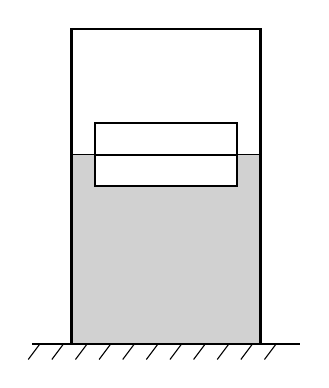
\begin{tikzpicture}[x=1cm,y=1cm]
\fill[black!18] (0,0) rectangle (2.4,2.4);
\draw[thick] (0,4)--(0,0)--(2.4,0)--(2.4,4)--cycle;
\draw (0,2.4)--(2.4,2.4);
\filldraw[fill=white,thick] (.3,2.0) rectangle (2.1,2.4);
\filldraw[fill=white,thick] (.3,2.4) rectangle (2.1,2.8);
\draw[thick] (-.5,0)--(2.9,0);
\foreach \x in {-.4,-.1,.2,.5,.8,1.1,1.4,1.7,2,2.3,2.6} \draw (\x,0)--++(-.15,-.2);
\end{tikzpicture}\end{center}
\begin{enumerate}
\item Если воду заменить на керосин, то глубина погружения брусков уменьшится.
\item Сила Архимеда, действующая на бруски, равна $20\,\text{Н}$.
\item Плотность материала, из которого изготовлены бруски, равна $500\,\text{кг}/\text{м}^{3}$.
\item Если на верхний брусок положить груз массой $0{,}7\,\text{кг}$, то бруски утонут.
\item Если в стопку добавить ещё два таких же бруска, то глубина её погружения увеличится на $10\,\text{см}$.
\end{enumerate}
}{
\smallskip\noindent\textbf{Решение от GPT}\par
$F_A=2mg=20\,\text{Н}$. Погружена половина суммарного объёма, поэтому $\rho_{\text{б}}=\rho_{\text{в}}/2=500\,\text{кг}/\text{м}^3$. В керосине погружение увеличится. Максимальная поддерживаемая масса $4\,\text{кг}$, поэтому груз $0{,}7\,\text{кг}$ не утопит систему. При добавлении ещё двух брусков погруженная толщина возрастёт с $5$ до $10\,\text{см}$, то есть на $5\,\text{см}$. Ответ: $23$.
}

% Source CCDA00: https://ege.fipi.ru/bank/questions.php?search=1&proj=BA1F39653304A5B041B656915DC36B38&qid=CCDA00
\BankTask{CCDA00}{
На поверхности воды плавает прямоугольный брусок из древесины плотностью $400\,\text{кг}/\text{м}^{3}$. Брусок заменили на другой брусок той же массы и с той же площадью основания, но из древесины плотностью $600\,\text{кг}/\text{м}^{3}$. Как при этом изменились глубина погружения бруска и действующая на него сила Архимеда?
\begin{enumerate}
\item увеличилась
\item уменьшилась
\item не изменилась
\end{enumerate}
\TaskChangeTable{Глубина погружения бруска}{Сила Архимеда}
}{
\smallskip\noindent\textbf{Решение от GPT}\par
При плавании $F_A=mg$, а $\rho_{\text{воды}}gSh=mg$. При одинаковых $m,S$ обе величины неизменны: $h=m/(\rho_{\text{воды}}S)$. Ответ: $33$.
}

% Source E2791B: https://ege.fipi.ru/bank/questions.php?search=1&proj=BA1F39653304A5B041B656915DC36B38&qid=E2791B
\BankTask{E2791B}{
На поверхности подсолнечного масла плавает деревянный шарик, частично погружённый в жидкость. Как изменятся сила Архимеда, действующая
на шарик, и глубина погружения шарика, если он будет плавать в воде?
\begin{enumerate}
\item увеличится
\item уменьшится
\item не изменится
\end{enumerate}
\TaskChangeTable{Сила Архимеда}{Глубина погружения шарика в жидкость}
}{
\smallskip\noindent\textbf{Решение от GPT}\par
При плавании $F_A=mg$ не меняется. Плотность воды больше плотности масла, поэтому $V_{\text{погр}}=m/\rho$ и глубина погружения уменьшаются. Ответ: $32$.
}

% Source 10BE25: https://ege.fipi.ru/bank/questions.php?search=1&proj=BA1F39653304A5B041B656915DC36B38&qid=10BE25
\BankTask{10BE25}{
На поверхности пресной воды плотностью $\rho_{1}=1000\,\text{кг}/\text{м}^{3}$ плавает деревянный брусок. Как изменятся масса вытесненной бруском жидкости и действующая на него сила Архимеда, если этот брусок будет плавать на поверхности керосина плотностью $\rho_{2}=800\,\text{кг}/\text{м}^{3}$?
\begin{enumerate}
\item увеличится
\item уменьшится
\item не изменится
\end{enumerate}
\TaskChangeTable{Масса вытесненной бруском жидкости}{Сила Архимеда}
}{
\smallskip\noindent\textbf{Решение от GPT}\par
При плавании $F_A=mg$, а масса вытесненной жидкости $m_{\text{ж}}=F_A/g=m$. Обе величины не зависят от плотности жидкости и не изменяются. Ответ: $33$.
}

% Source 38974: https://phys-ege.sdamgia.ru/problem?id=38974
\BankTask{38974}{
Деревянный шар привязан нитью ко дну цилиндрического сосуда с площадью дна S  =  $200\,\text{см}^{2}$. В сосуд наливают воду так, что шар полностью погружается в жидкость, при этом нить натягивается и действует на шар с силой T. Если нить перерезать, то шар всплывёт, а уровень воды изменится на h  =  $5\,\text{см}$. Найдите силу натяжения нити T.
}{
\smallskip\noindent\textbf{Решение}\par
В первом случае на шар действуют сила натяжения нити T и сила тяжести mg, направленные вертикально вниз, сила Архимеда $F_{A1},$ направленная вертикально вверх. Во втором случае на него действуют сила тяжести и сила Архимеда $F_{A2}$ при частичном погружении шара. Запишем второй закон Ньютона для каждого случая при ускорении, равном $0$:

$F_{A1} - mg - T=0,$
$F_{A2} - mg=0.$

В первом случае шар погружен полностью в воду, поэтому $F_{A1}=\rho gV,$ где V  — объем шара. Во втором случае шар погружен частично, поэтому $F_{A2}=\rho gV_{\,\text{пчт}},$ где V$_{\,\text{пчт}}$  — объем погруженной части шара.
Так как по закону Архимеда объем вытесненной жидкости равен объему погруженной части тела, то при его изменении меняется объем жидкости в сосуде на величину $\Delta V=V - V_{\,\text{пчт}}.$
Если обозначить h$_{1}$  — уровень воды в сосуде в первом случае, h$_{2}$  — уровень воды в сосуде во втором случае, то изменение уровня воды равно $h=h_1 - h_2.$ Тогда объем вытесненной воды при всплывании шара изменился на $\Delta V=Sh.$
Объединяя уравнения, находим силу натяжения нити:

\[T=\rho gSh=10 ^3 \cdot 10 \cdot 200 \cdot 10 ^{ - 4 } \cdot 5 \cdot 10 ^{ - 2 } =10\,\text{Н}.\]

Ответ: $T=10\,\text{Н}.$
}

% Source 50850: https://phys-ege.sdamgia.ru/problem?id=50850
\BankTask{50850}{
\begin{center}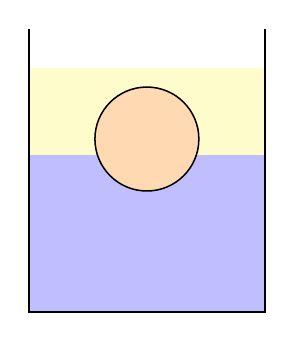
\begin{tikzpicture}[>=stealth,line width=.55pt]\fill[blue!25](0,0)rectangle(3,2);\fill[yellow!20](0,2)rectangle(3,3.1);\draw[thick](0,3.6)--(0,0)--(3,0)--(3,3.6);\draw[fill=orange!30](1.5,2.2)circle(.66);\end{tikzpicture}\end{center}В стакан налита вода, а поверх неё  — керосин. Однородный шар плавает, погружённый в обе жидкости. При этом $\frac{1}{6}$ объёма шара находится в воде, а $\frac{5}{6}$ объёма  — в керосине. Найдите плотность материала шара.
}{
\smallskip\noindent\textbf{Решение}\par
На шар действуют три силы: силы Архимеда со стороны керосина и воды, направленные вертикально вверх и сила тяжести, направленная вертикально вниз. Так как шар плавает, то выполняется условие равновесия:

\[F_{A1} + F_{A2}=mg.\]

Сила Архимеда со стороны керосина $F_{A1}= \frac{5}{6} \rho_{\,\text{к}}gV,$ сила Архимеда со стороны воды $F_{A2}= \frac{1}{6} \rho_{\,\text{в}}gV,$ масса тела $m=\rho V,$ где V  — объем тела. При объединении уравнений находим плотность материала шарика:

\[\rho= \frac{5\rho_{\,\text{к}} + \rho_{\,\text{в}}}{6} = \frac{5 \cdot 800 + 1000}{6} \approx 833 \,\text{кг/м} ^3 .\]

Ответ: $\approx 833 \,\text{кг/м} ^3 .$
}

\end{document}
